\documentclass[../main]{subfiles}
\begin{document}

\section{Gestione di progetto}
Sono state presentate in §1 e in §2 due descrizioni della parola \g{progetto}: una secondo Kerzner, una secondo il SEMAT. Entrambe si rapportano con il \g{ciclo di vita del prodotto software}.
Gestire un \g{progetto} significa:
\begin{itemize}
    \item Istanziare processi (come in §2.5);
    \item Stimare costi e risorse necessarie;
    \item Pianificare le attività e assegnarle alle persone (come detto in §1, si pianifica dalla fine e non dall'inizio);
    \item Controllare l'andamento delle attività e verificarne i risultati frequentemente (vanno prevenute le situazioni di errore).
\end{itemize}
\subsection{Ruoli di progetto}
Un \g{ruolo} è una responsabilità che viene data ad una persona che dipende dal \g{processo} in cui essa opera. Ad un ruolo tipicamente corrisponde un profilo professionale, ovvero l'insieme delle competenze tecnologiche e metodologiche che una persona ha maturato partecipando a progetti e che può usare per soddisfare dei requisiti quando richiesti.\newline
Nel settore IT non c'è ancora la possibilità di avere un ruolo professionale fisso, quasi sempre i ruoli variano in base alle necessità. I ruoli in un \g{progetto} software sono:
\begin{itemize}
    \item Analista: figura che conosce il \g{dominio} del problema e ha esperienza professionale. Il suo lavoro è la base per tutto ciò che verrà svolto successivamente, per cui il suo lavoro è essenziale che sia il più possibile accurato. Non ha la necessità di seguire il \g{progetto} fino alla fine e spesso scarseggia (ovvero, ci sono pochi analisti);
    \item Progettista: figura che ha competenze tecniche e metodologiche per riprendere il lavoro dell'analista e strutturarlo per creare le basi per lo sviluppo successivo. Ha molto peso poiché dalle sue scelte dipende l'implementazione del \g{prodotto software}. Anch'esso scarseggia ma segue comunque il \g{progetto} per tutto lo sviluppo, per poi abbandonarlo per la manutenzione;
    \item Programmatore: figura che partecipa sia alla realizzazione (implementazione) del prodotto software che alla manutenzione. Ha competenze tecniche per poter concretizzare il lavoro del progettista ma le sue responsabilità sono circoscritte, così come la propria libertà d'azione. Storicamente è il ruolo più numeroso;
    \item Verificatore: figura che partecipa per l'intera durata del \g{progetto} ed è fondamentale, poiché possiede sia le competenze tecniche, l'esperienza maturata e la conoscenza delle norme da attuare per verificare se ciò che viene svolto è corretto, potendo quindi dare dei giudizi critici;
    \item Responsabile: figura che si assume l'onore di rappresentare il \g{progetto} presso il fornitore e il committente. Ha libertà e responsabilità di scelta e approvazione. Le sue responsabilità ricadono sulla pianificazione, gestione delle risorse, controllo e coordinamento. Deve avere conoscenze e capacità tecniche per poter giudicare e valutare i rischi e fornire alternative;
    \item Amministratore: figura che controlla l'ambiente di lavoro, amministra le infrastrutture di supporto e risolve i problemi nella gestione dei processi. Gestisce la documentazione e il controllo di versione e configurazione. Tipicamente non è un ruolo solamente di \g{progetto}, ma è più aziendale.
\end{itemize}
\subsection{Gestione qualità}
La gestione della qualità è fondamentale per un \g{progetto} software, anche se è più una funzione aziendale che di progetto. Infatti, non basta solamente il ruolo del verificatore, che è tipicamente retrospettivo.\newline
Essa riguarda sia i processi che i prodotti ed è interesse di tutti coloro che lavorano al progetto di perseguirla.
\subsection{Pianificazione di progetto}
La pianificazione del progetto include le seguenti attività:
\begin{itemize}
    \item Pianificazione dello svolgimento dei processi e delle loro attività, e controllarne l'andamento;
    \item Non c'è nulla da inventare, le attività devono seguire un certo ordine in base alle pre-condizioni e post-condizioni di ogni attività;
    \item Ogni attività ha bisogno delle proprie risorse e ha i propri costi e le proprie scadenze;
    \item Identificazione dei ruoli di progetto e assegnazione dei ruoli alle persone, senza sottostimare e sovrastimare.
\end{itemize}
A supporto della pianificazione ci sono vari strumenti, tra cui:
\begin{itemize}
    \item Diagramma di Gantt
    \item \textit{Programme Evaluation and Review Technique} (PERT)
    \item Work Breakdown Structure (WBS)
\end{itemize}
\subsubsection{Diagramma di Gantt}
Diagramma utilizzato per decidere e visualizzare la dislocazione temporale delle attività. In questo tipo di diagramma è possibile osservare la durata di un'attività, la posizione in cui si trova nell'intera sequenza di attività da svolgere e anche con quali altre viene eseguita in parallelo. Infine, permette di controllare quanto la stima di una durata sia stata corretta confrontandola con il progresso reale.
\begin{figure}[h]
    \begin{center}
        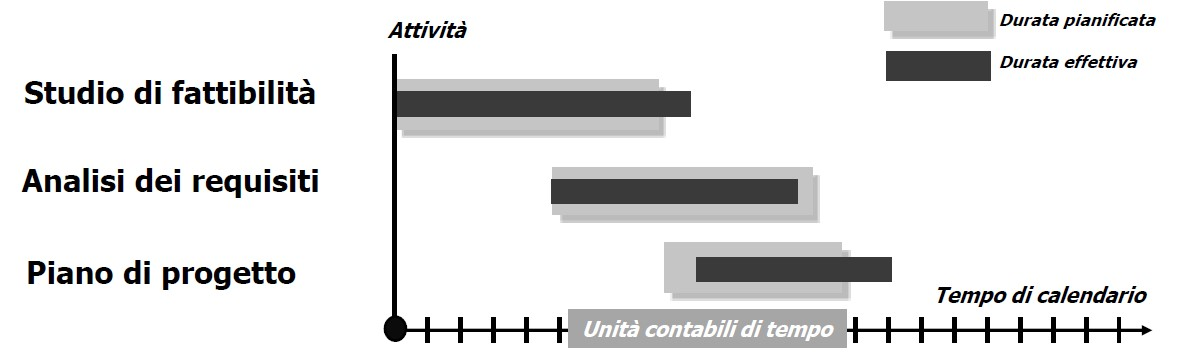
\includegraphics[scale=0.5]{immagini/gantt.jpg}
    \end{center}
\end{figure}
\subsubsection{Programme Evaluation and Review Technique (PERT)}
Diagramma utilizzato per ragionare (all'indietro) sulle scadenze. Si basa sul concetto di \textit{slack}, ovvero sullo scarto che ho fra la fine di un'attività e l'inizio della successiva. Lo slack non deve essere troppo basso (tendente a 0) altrimenti si rischia di andare negativi (\textit{"attività da finire per ieri"}) ma nemmeno troppo alto perché potrebbe segnalare inattività.
\begin{figure}[h]
    \begin{center}
        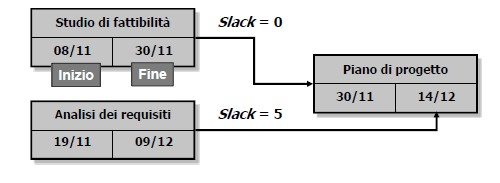
\includegraphics[scale=0.8]{immagini/pert.jpg}
    \end{center}
\end{figure}
\subsubsection{Work Breakdown Structure (WBS)}
Diagramma che rappresenta le attività da svolgere come struttura gerarchica. Ad ogni attività è assegnato un codice univoco, e ogni attività è formata di sotto-attività, non necessariamente sequenziali, che la completano.
\begin{figure}[h]
    \begin{center}
        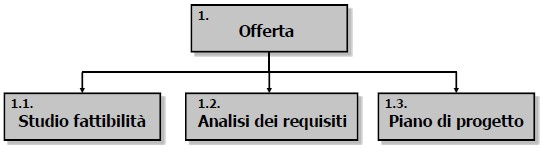
\includegraphics[scale=0.8]{immagini/wbs.jpg}
    \end{center}
\end{figure}
\end{document}